
\begin{frame}
	\frametitle{OK???}
	
	Vérifions d'abord que la méthode est bien définie.
	
	\mbox{}
	
	{\red Justification de l'étape 1}
	
	\mbox{}
	
	Nous avons supposé le problème résolvable. Par le théorème précédent
	(optimalité LP)
	\begin{align*}
		\lbrace (x,y) \,|\, Ax = b,\ Tx+Wy = h,\ x \geq 0,\ y \geq 0\rbrace \ne
		\emptyset,\\
		\lbrace v \,|\, Wv = 0,\ q^Tv < 0,\ v \geq 0 \rbrace = \emptyset.
	\end{align*}
	De plus, $\lbrace x \,|\, Ax = b,\ x \geq 0 \rbrace$ est fermé et
	borné. Dès lors
	$\inf \lbrace f(x) \,|\, Ax = b,\ x \geq 0 \rbrace$ est fini (fonction
	continue sur un ensemble non vide compact) et il
	existe une borne inférieure $\theta_0$ pour $f(x)$.
	
	Par conséquent, le problème
	\[
	\min \lbrace c^Tx + \theta \,|\, Ax = b,\ \theta \geq \theta_0,\ x
	\geq 0 \rbrace
	\]
	peut être résolu.
	
\end{frame}

\begin{frame}
	\frametitle{Rappel (encore!): relativement complet}
	
	Caractérisation du recours relativement complet:
	\[
	h(\xi) - T(\xi)x \in \mbox{pos}W \mbox{ pour tout } \xi \mbox{ et tout
	}x \geq 0 \mbox{ t.q. } Ax=b,
	\]
	\[
	\mbox{où pos}W = \lbrace t \,|\, t = Wy,\ y \geq 0 \rbrace.
	\]
	En d'autres termes, $h(\xi) - T(\xi)x$ est une combinaison linéaire
	positive (non-négative) des colonnes de $W$.
	
	\begin{block}{Proposition}
		L'ensemble $pos W$
		est un cône convexe polyhédrale.
	\end{block}
	
	\begin{itemize}
		\item
		Cône convexe: toute combinaison convexe de deux éléments de
		$\mathcal{C}$ est un élément de $\mathcal{C}$. Evident (exercice!).
	\end{itemize}
	
	
\end{frame}

\begin{frame}
	\frametitle{pos $W$}
	
	\begin{itemize}
		\item
		cône convexe polyhédral: il existe un nombre fini de vecteurs
		$t^{\lbrace i \rbrace} \in \mbox{pos}W$, $i = 1,\ldots,r$, tel que
		n'importe quel $t \in \mbox{pos}W$ peut être représenté comme
		\[
		t = \sum_{i=1}^r \alpha_i t^{\lbrace i \rbrace},\ \alpha_i \geq 0\
		\forall i.
		\]
		Il suffit de prendre les colonnes de $W$ comme $t^{\lbrace i \rbrace}$!
	\end{itemize}
	
	%\begin{block}{Proposition}
	%L'ensemble $\mathcal{C} := \lbrace y \,|\, 0 = Wy,\ y \geq 0 \rbrace$
	%est un cône convexe polyhédrale.
	%\end{block}
	
\end{frame}

\begin{frame}
	\frametitle{Problème de deuxième étape}
	
	\[
	Q(x,\xi){=} \min \lbrace q(\xi)^Ty \ |\ Wy = h(\xi) - T(\xi)x,\ y \geq 0 \rbrace.
	\]
	
	\mbox{}
	
	Du lemme de Farkas, on avait vu que le problème de seconde étape est
	réalisable si et seulement si $z^Tt \leq 0$ quand 
	\[
	t \in \mbox{pol pos} W =
	\lbrace u \,|\, u^Tz \leq 0\ \forall z \in \mbox{pos} W \rbrace.
	\]
	
	\mbox{}
	
	En d'autres termes, le système $Wy = z$, $z \geq 0$, est réalisable si
	et seulement le terme de droite $z$ a un produit scalaire non-positif
	avec tous les vecteurs du cône $\mbox{pol pos} W$.
	
	\mbox{}
	
	De la même manière que pour pos$W$, on peut construire les éléments
	générateurs de pol pos$W$ et construire la matrice $W^*$ en utilisant
	ces générateurs comme colonnes de $W^*$.
\end{frame}

\begin{frame}
	\frametitle{Coupes de faisabilité}
	
	Dès lors, si nous connaissions $W^*$, nous pourrions vérifier la
	faisabilité du problème de seconde étape.
	
	\mbox{}
	
	Comme généralement, ce n'est pas le cas, nous devons vérifier la
	faisabilité pour un $\hat{x}$ donné et tout $\xi \in \mathcal{A}$.
	
	Idée: obtenir un générateur de pol pos$W$  si le problème donné n'est
	pas réalisable.
	
	\mbox{}
	
	Nous souhaiterions trouver un $\sigma$ dans pol pos$W$, i.e.
	\[
	\sigma^Tt \leq 0 \mbox{ pour tout } t \in \mbox{pos }W,
	\]
	autrement dit tel que $\sigma^TW \leq 0$.
	
\end{frame}

\begin{frame}
	\frametitle{Coupes de faisabilité (2)}
	
	{\red Hypothèse:} $h(\xi) - T(\xi)\hat{x}$ produit un problème
	irréalisable.\\
	Dans ce cas, nous devrions avoir
	\[
	\sigma^T(h(\xi) - T(\xi)\hat{x}) > 0.
	\]
	Ainsi, en ajoutant la contrainte
	\[
	\sigma^T(h(\xi) - T(\xi) x) \leq 0,
	\]
	nous excluons le membre de droite irréalisable $h(\xi) -
	T(\xi)\hat{x}$ sans rejeter de solutions réalisables.
	
	\begin{center}
		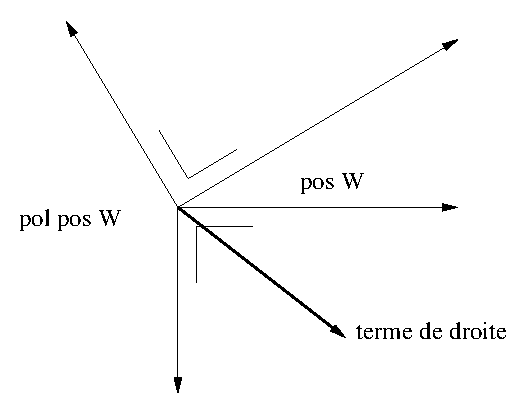
\includegraphics[width=0.45\textwidth]{cones_2.eps}
	\end{center}
	
\end{frame}

\begin{frame}
	\frametitle{Coupes de faisabilité (3)}
	
	Dès lors, nous souhaitons résoudre
	\[
	\max_{\sigma} \lbrace \sigma^T(h(\xi) - T(\xi)\hat{x}) \,|\, \sigma^TW
	\leq 0,\ \|\sigma\| = 1 \rbrace.
	\]
	$\sigma$ est borné pour éviter d'aller à l'infini. Idéalement,
	nous devrions utiliser la norme 2, mais pour des raisons
	computationnelles, nous utiliserons la norme 1 (voir exemple 3.1 de
	Kall et Wallace).
	
	\mbox{}
	
	%Remplaçons $\sigma$ par $\sigma_1,\ \sigma_2 \geq 0$:
	%\begin{align*}
	%\max_{\sigma} \lbrace & (\sigma_1 - \sigma_2)^T(h(\xi) - T(\xi)\hat{x})
	%\,|\, (\sigma_1-\sigma_2)^TW \leq 0,\\
	%& e^T(\sigma_1+\sigma_2) \leq 1, \sigma_1, \sigma_2 \geq 0 \rbrace,
	%\end{align*}
	%où $e = (1,\ldots,1)^T$.
	
	Le dual s'exprime comme
	\begin{align*}
		\min & \lbrace v \,|\, Wy + Iv = h(\xi) - T(\xi)\hat{x},\ y, v \geq 0 \rbrace.
	\end{align*}
	Si $v^* = 0$, $Wy = (h(\xi) - T(\xi)\hat{x})$, autrement dit $(h(\xi) -
	T(\xi)\hat{x}) \in \mbox{pos}W$, contrairement à notre hypothèse.
	
	Mais pour $v$ assez grand, le problème est réalisable.
	
\end{frame}

\begin{frame}
	\frametitle{Coupes de faisabilité (4)}
	
	Nous devons résoudre ce problème pour tout $\xi$.
	Si pour un certain $\xi$ nous obtenons une valeur optimale strictement
	positive, nous créons la coupe
	\[
	\sigma^T(h(\xi)-T(\xi)x) \leq 0.
	\]
	ou encore
	\[
	Dx \geq d,
	\]
	avec $D = \sigma^TT(\xi)$ et $d = \sigma^Th(\xi)$.
	%$\sigma$ est un générateur de pol pos$W$, mais n'est pas aussi proche
	%du membre de $z$ que possible.
	
	\mbox{}
	
	Via la programmation linéaire, on peut montrer qu'il y a un nombre
	fini de base optimales au sous-problème servant à produire les coupes
	de faisabilité.
	\mbox{}
	
	En fait, on peut aussi montrer que si $\bxi$ est une variable aléatoire
	finie, $K_2$ est polyhédral.
	
\end{frame}

\begin{frame}
	\frametitle{Types de recours}
	
	Définissons le cône pos$W$ par
	\[
	\mbox{pos}W = \lbrace t \,|\, t = Wy,\ y \geq 0 \rbrace.
	\]
	Cône: $\forall\, t \in \mbox{pos}W,\ \alpha > 0$, $\alpha t \in  \mbox{pos}W$.
	
	\mbox{}
	
	Nous avons
	\[
	Wy = t,\ y \geq 0 \mbox{ est réalisable ssi } t \in \mbox{pos}W.
	\]
	
	\mbox{}
	
	{\red Recours complet}: {\blue pos$W = \rit^m$}.
	Ceci implique
	\[
	h(\omega) - T(\omega)x \in \mbox{pos}W \ \forall\, \omega, x.
	\]
	
	\mbox{}
	
	{\red Recours relativement complet}:
	\[
	h(\omega) - T(\omega)x \in \mbox{pos}W \mbox{ pour tout } \omega \mbox{ et tout
	}x \geq 0 \mbox{ t.q. } Ax=b.
	\]
	
\end{frame}

\begin{frame}
	\frametitle{Recours relativement complet}
	
	Comment identifier le recours relativement complet?
	
	\mbox{}
	
	Utilisation du lemme de Farkas: condition nécessaire et suffisante
	pour la faisabilité d'un système d'équations linéaires.
	
	\begin{block}{Lemme de Farkas}
		$\lbrace x \,|\,  Ax = b,\ x \geq 0 \rbrace \ne \emptyset$
		si et seulement si
		\[
		A^Tu \geq 0 \mbox{ implique } b^Tu \geq 0.
		\]
	\end{block}
	
	\mbox{}
	
	Recours relativement complet: $z \in \mbox{pos} W$ ou $\lbrace y \,|\,
	Wy = z,\ y \geq 0\rbrace \ne \emptyset$.
	
	Par le lemme de Farkas, cela équivaut à
	$(W^Tu \geq 0) \Rightarrow (z^Tu \geq 0).$
	
\end{frame}

\begin{frame}
	\frametitle{Implications du lemme de Farkas}
	
	Par conséquent, $(-W^Tu \geq 0) \Rightarrow (-z^Tu \geq 0)$, ou 
	$(W^Tu \leq 0) \Rightarrow (z^Tu \leq 0)$,
	ou encore
	\[
	z^Tt \leq 0 \mbox{ quand } t \in \lbrace u \,|\, W^Tu \leq 0\rbrace.
	\]
	
	\mbox{}
	
	Or, par définition du produit scalaire, 
	\[
	\lbrace u \,|\, W^Tu \leq 0 \rbrace = \lbrace u \,|\, y^TW^Tu \leq 0\ \forall y \geq 0 \rbrace
	\]
	ou encore, par défintion de pos$W$,
	\[
	\lbrace u \,|\, W^Tu \leq 0 \rbrace
	= \lbrace u \,|\, u^TWy \leq 0\ \forall y \geq 0 \rbrace
	= \lbrace u \,|\, u^Tz \leq 0\ \forall z \in \mbox{pos} W \rbrace.
	\]
	
	Cette dernière expression définit le {\blue cône polaire} de pos$W$:
	\[
	\mbox{pol pos} W =
	\lbrace u \,|\, u^Tz \leq 0\ \forall z \in \mbox{pos} W \rbrace.
	\]
	Le lemme de Farkas va nous être utile pour vérifier et {\red forcer} le recours relativement
	complet.
	
\end{frame}

\begin{frame}
	\frametitle{Justification: détour par la programmation linéaire}
	
	Considérons le système $Ax = b$. Comme précédemment, nous supposerons
	que $rang(A) = m$, et l'ensemble réalisable du problème linéaire
	standard
	\[
	\mathcal{B} = \lbrace x \,|\, Ax=b,\ x \geq 0 \rbrace.
	\]
	
	\mbox{}
	
	{\red Solution réalisable de base}: $\hat{x} \in \mathcal{B}$
	(faisabilité), et soit $I(\hat{x}) = \lbrace i \,|\, \hat{x}_i > 0
	\rbrace$, l'ensemble $\lbrace A_i \,|\, i \in I(\hat{x}) \rbrace$ de
	colonnes de $A$ est linéairement indépendant.
	
	\mbox{}
	
	Les composantes $\hat{x}_i$, $i \in I(\hat{x})$, sont l'unique
	solution du système
	\[
	\sum_{i \in I(\hat{x})} A_ix_i = b.
	\]
	
\end{frame}

%\begin{frame}
%\frametitle{LP: ensemble réalisable}

%\begin{block}{Proposition}
%Si $\mathcal{B}$ est un ensemble borné et $\mathcal{B} \ne \emptyset$,
%alors $\mathcal{B}$ est l'enveloppe convexe (i.e. l'ensemble de toutes
%les combinaisons convexes) de l'ensemble de ses solutions de base
%réalisables.
%\end{block}

%\end{frame}


\begin{frame}
	\frametitle{LP: solution de base optimale}
	
	\begin{theo}[Optimalité LP]
		Considérons le problème linéaire standard
		\begin{align*}
			\min\ & c^Tx \\
			\mbox{t.q. } & Ax = b,\ x \geq 0.
		\end{align*}
		Ce problème peut être résolu si et seulement si
		\[
		\mathcal{B} = \lbrace x \,|\, Ax = b,\ x \geq 0 \rbrace \ne \emptyset, \mbox{ faisabilité}
		\]
		et
		\[
		c^Ty \geq 0,\ \forall y \in \mathcal{C} = \lbrace y \,|\, Ay = 0,\ y \geq 0 \rbrace.
		\]
		Si ces deux conditions sont satisfaites, il y a au moins une solution
		réalisable de base qui est une solution optimale.
	\end{theo}
\end{frame}
